\documentclass[]{article}
\usepackage[hidelinks]{hyperref}
\usepackage{graphicx, amsmath, listings, amssymb, commath}
\usepackage[utf8]{inputenc}
\lstdefinestyle{mystyle}{
	showtabs=false, 
	tabsize=2
}

\lstdefinestyle{mystyle}{
	showtabs=false, 
	tabsize=2
}
\lstset{style=mystyle}
\usepackage[utf8]{inputenc}

\title{Rešitev 2. projektne naloge MM}
\author{Aljaž Verlič, Lina Lumborovska, Blažka Blatnik, Luka Tavčer \\
	Mentor: Damir Franetič}
\date{5. junij, 2017}

\begin{document}

\maketitle
\renewcommand{\abstractname}{Uvod}
%\begin{abstract}

%\end{abstract}

\section{Presek dveh implicitno danih ploskev}
	V $\mathbb{R}^3$ imamo podani dve poljubni implicitno podani ploskvi, opisanimi z enačbama $f_{1}(x)$ = $C_{1}$ in\\ $f_{2}(x)$ = $C_{2}$, presek pa je množica rešitev tega nelinearnega sistema enačb.\\
	Naša naloga je poiskati krivuljo $K$, ki predstavlja presek teh dveh ploskev. \\ \\
	Nalogo bomo rešili na 4 načine z uporabo metod za numerično reševanje diferencialnih enačb. Uporabili bomo:
	\begin{itemize}  
		\item Eulerjevo/Runge-Kutta s fiksno dolžino koraka
		\item Eulerjevo/Runge-Kutta z adaptivno dolžino koraka
	\end{itemize}

\subsection{Delovanje metode}
	

\subsection{Potrebni pogoj in Jacobijeva matrika}
	Potreben pogoj za delovanje metod je, da sta funkciji $f_{1}$ in $f_{2}$ parcialno odvedljivi in da ima Jacobijeva matrika parcialnih odvodov poln rang 2. Za uspešno delovanje Newtonove metode moramo poiskati Jacobijevo matriko leve strani sistema nelinearnih enačb.

	\begin{center}
		JG = $\begin{bmatrix}
		grad(f_{1}) \\
		grad(f_{2}) \\
		\hspace{1mm}grad(\vec{v} \cdot \vec{x}) \\
		\end{bmatrix}$
		oziroma
		JG = $\begin{bmatrix}
		grad(f_{1}) \\
		grad(f_{2}) \\
		\hspace{1mm}grad(\vec{v}\hspace{0.5mm}^\intercal) \\
		\end{bmatrix}$
	\end{center}
	%[x, k] = newton(G, JG, x0, tol, maxit) poisce priblizek 
	%x za resitev enacbe F(x) = 0 z Newtonovo metodo.
	%(k je stevilo korakov, ki jih metoda porabi.)
	%G... funkcija
	%JG... Jacobijeva matrika G
	%x0... zacetni priblizek
	%tol... zahtevana natancnost
	%maxit... najvecje stevilo iteracij
	\begin{lstlisting}[language=Octave]
		function [x, k] = newton(G, JG, x0, tol, maxit)
			for k = 1:maxit
				%Izvedemo en korak Newtonove metode...
				x = x0 - feval(JG, x0)\feval(G, x0);
				
				if(norm(x - x0) < tol)	% Je metoda ze konvergirala?
					break;
				end
				x0 = x;
			endfor
			% Izpis opozorila, ce zadnji priblizek ni znotraj tolerance.
			if(k == maxit)
				disp("Warning: The method did not converge after maxit iterations.")
			end
		endfunction
	\end{lstlisting} \ \\

	%\includegraphics[scale=0.5]{sim_10x}

		
\subsection{Implementacija, testiranje in ugotovitve}
	Delovanje našega programa lahko preverimo s programom, ki smo ga napisali v Octave-u. Kot vhodne parametre mu podamo obe implicitno podani funkciji $f_{1}$, $f_{2}$, $C1$, $C2$, $grad(f_{1})$, $grad(f_{2})$. Določimo tudi začetni približek $x_{0}$, začetno dolžino koraka in pa parameter, ki določa metodo delovanja (Euler/Runge-Kutta).\\
	Program poženemo na različnih primerih in štejemo povprečno dolžino koraka ter število porabljenih korakov.\\
	Primer 1:
	\begin{itemize} 
		\item $f_{1}(x,y,z)$ = $x^2 + y^2 + z^2$ = 4
		\item $f_{2}(x,y,z)$ = $3x + 2y + z$ = 1	
	\end{itemize}
	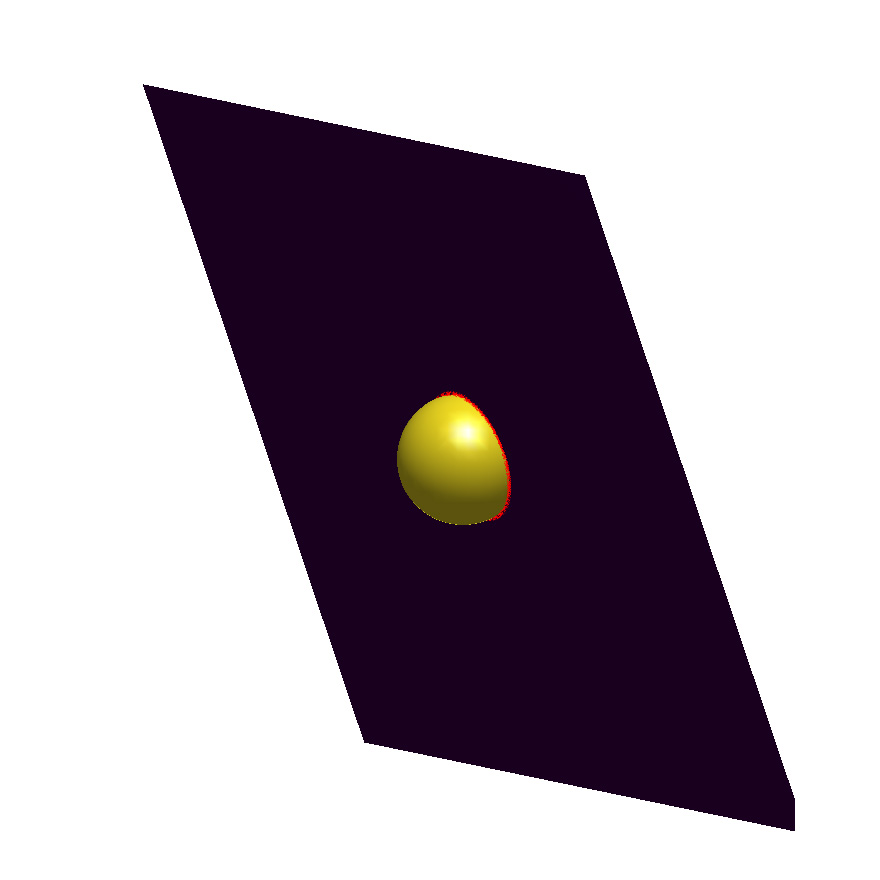
\includegraphics[scale=0.3]{primer1_1}
	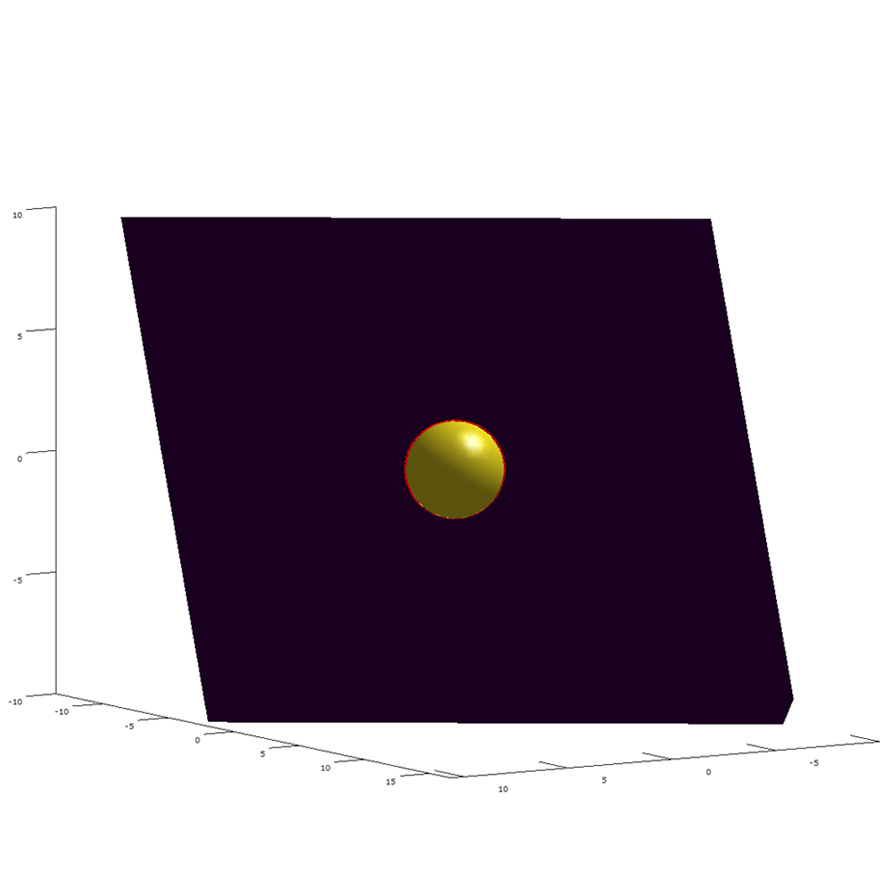
\includegraphics[scale=0.3]{primer1_2}
	VSTAVI TABELO REZULTATOV\\ \\
	Primer 2:
	\begin{itemize}  
		\item $f_{1}(x,y,z)$ = $x^2 + y^2 + z^2$ = 4
		\item $f_{2}(x,y,z)$ = $x^2 + y^2$ = 1
	\end{itemize}
	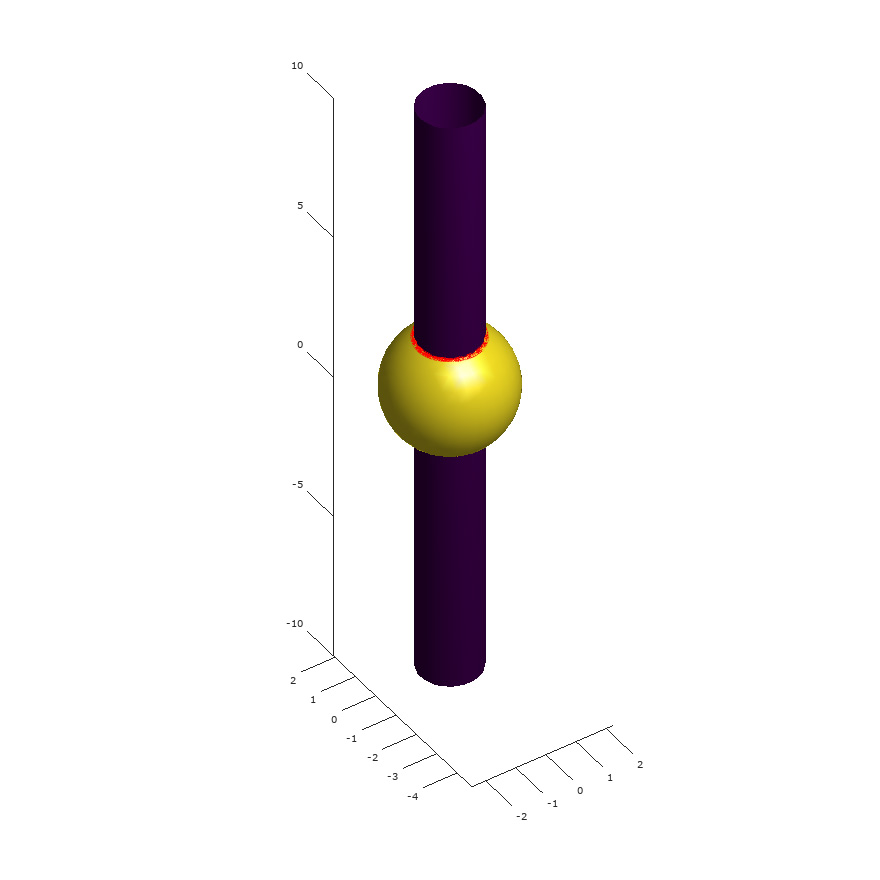
\includegraphics[scale=0.3]{primer2_1}
	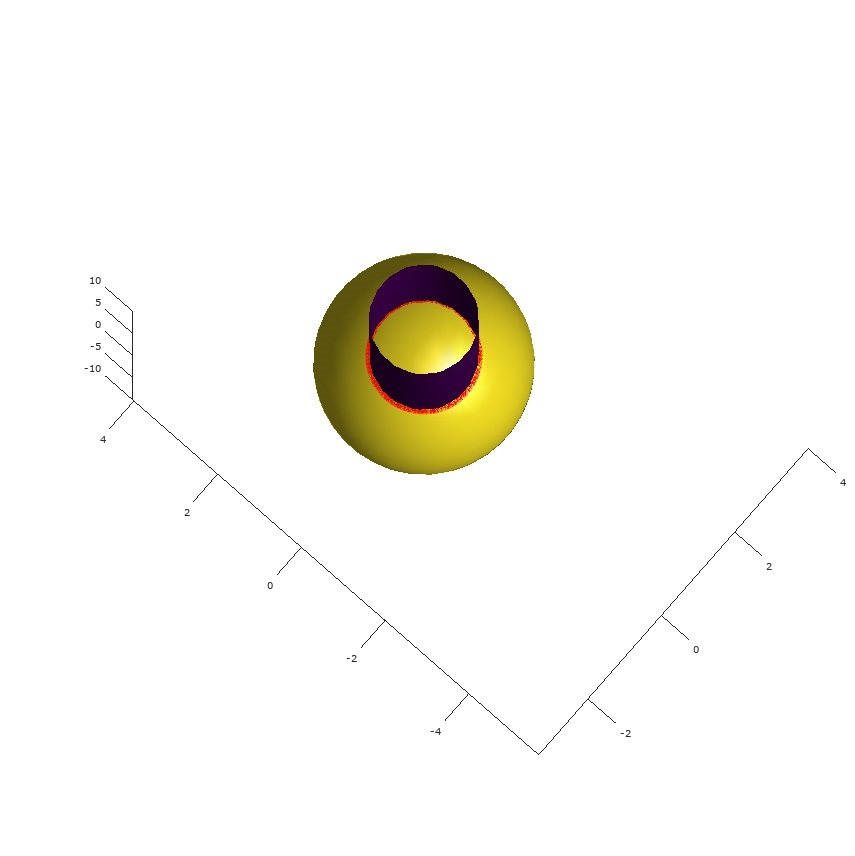
\includegraphics[scale=0.3]{primer2_2}
	VSTAVI TABELO REZULTATOV\\ \\
	Primer 3:
	\begin{itemize}  
		\item $f_{1}(x,y,z)$ = $x^2 + y^2 + z^2$ = 4
		\item $f_{2}(x,y,z)$ = $y^4 + log(x^2 + 1)z^2 - 4$ = 1
	\end{itemize}
	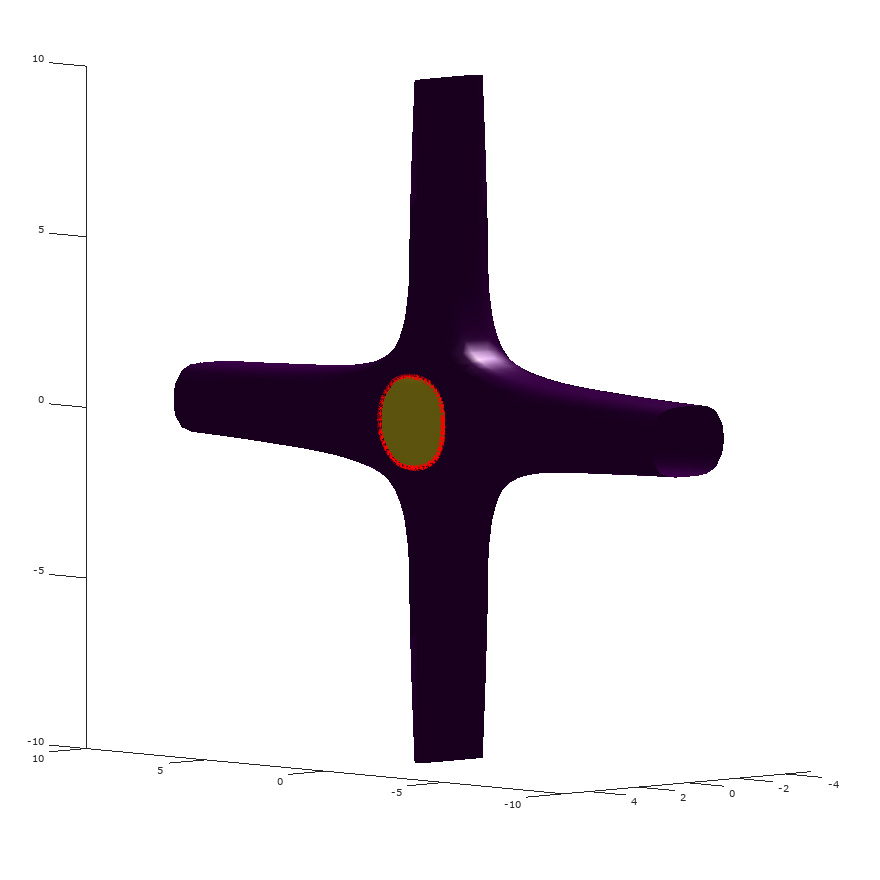
\includegraphics[scale=0.3]{primer3_1}
	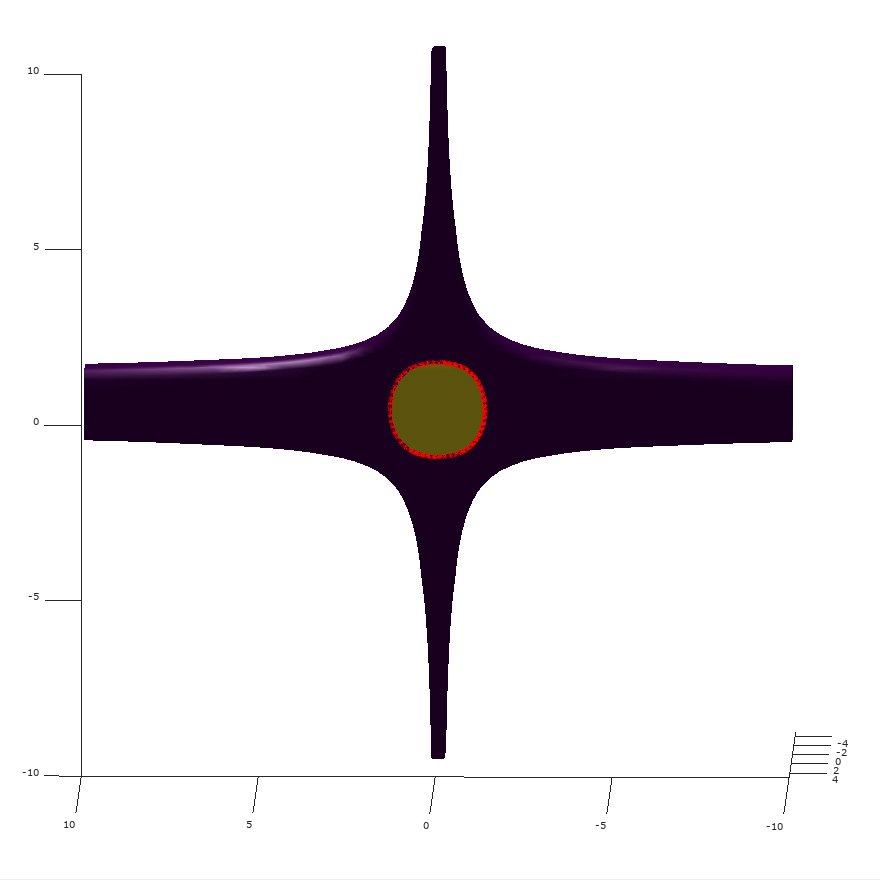
\includegraphics[scale=0.3]{primer3_2}
	VSTAVI TABELO REZULTATOV\\ \\
	Primer 4:
	\begin{itemize}  
		\item $f_{1}(x,y,z)$ = $x^2 + cos(y)z^2 - 12$ = 4
		\item $f_{2}(x,y,z)$ = $y^4 + log(x^2 + 1)z^2 - 4$ = 1
	\end{itemize}
	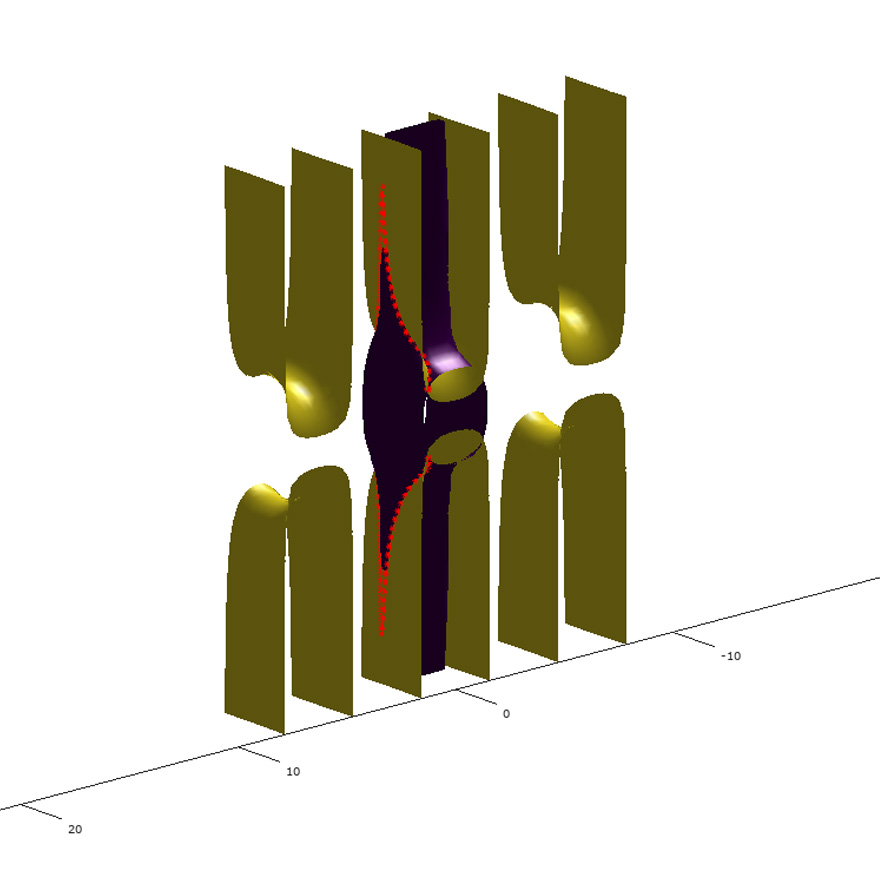
\includegraphics[scale=0.3]{primer4_1}
	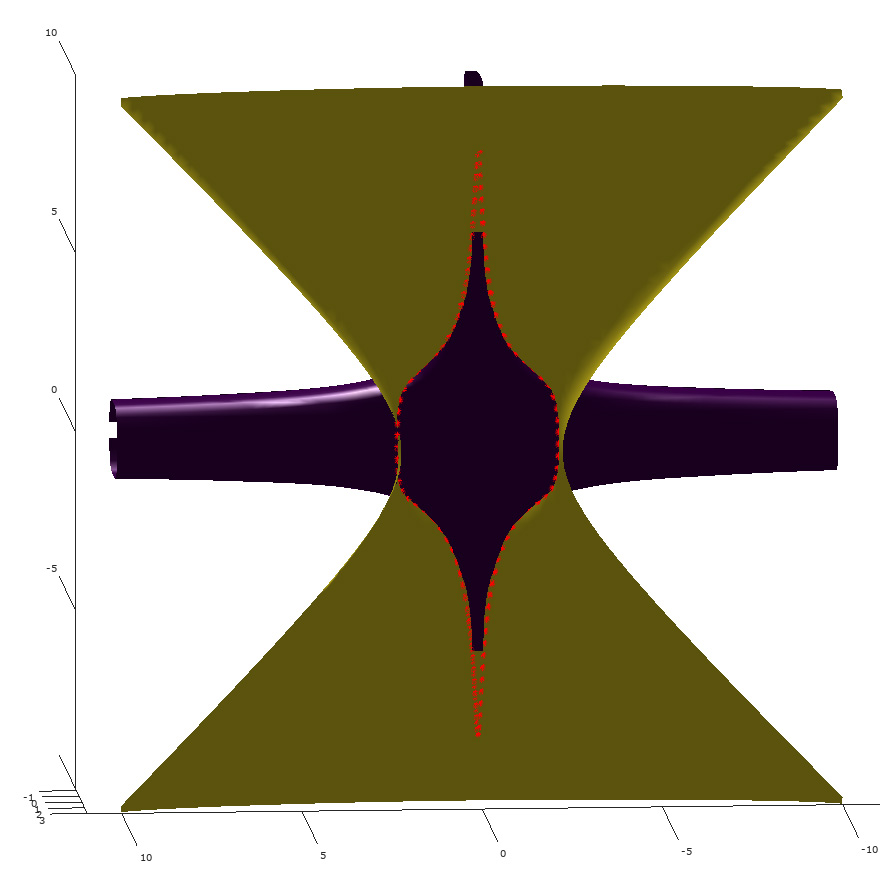
\includegraphics[scale=0.3]{primer4_2}
	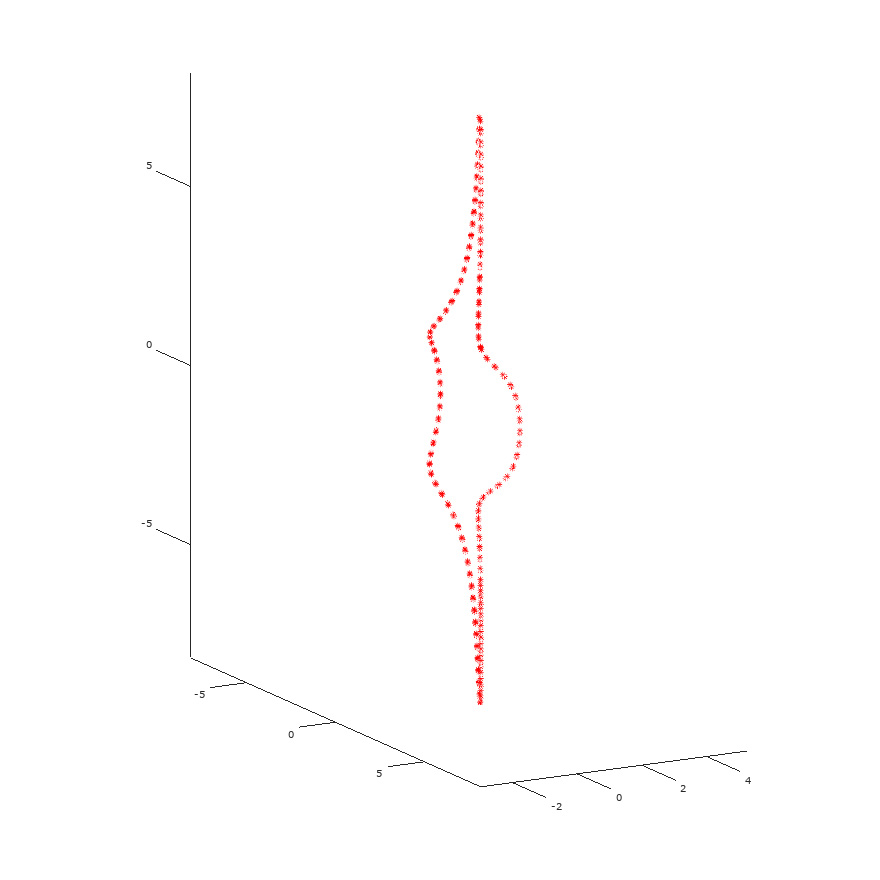
\includegraphics[scale=0.3]{primer4_4}
	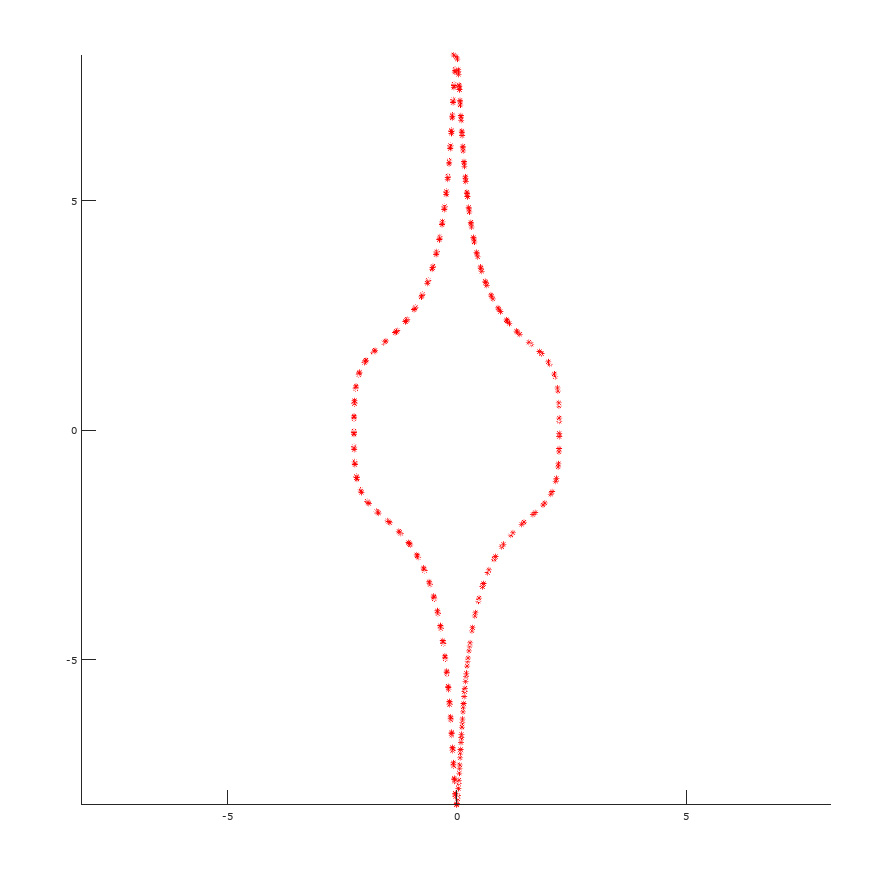
\includegraphics[scale=0.3]{primer4_3}
	VSTAVI TABELO REZULTATOV\\ \\

\end{document}
